\documentclass[UTF8,a4paper,10pt]{ctexart}
\usepackage[margin=19mm,top=20mm,bottom=19mm]{geometry}
\usepackage{amsmath,amssymb,booktabs,tabularx,graphicx,xcolor,fancyhdr,enumitem,tikz}
\usetikzlibrary{arrows.meta,positioning}
\usepackage[colorlinks=true,linkcolor=teal,urlcolor=teal]{hyperref}
\definecolor{ink}{HTML}{142B43}\definecolor{accent}{HTML}{168579}\definecolor{teal}{HTML}{168579}
\pagestyle{fancy}\fancyhf{}\fancyhead[L]{\small CF2026 Project 1}\fancyhead[R]{\small 青序量化研究平台}
\fancyfoot[L]{\scriptsize 平台 V230 / v2.3.0 / 2026-10-01 · 固定历史快照 · 描述性结果}\fancyfoot[R]{\thepage/10}
\setlength{\headheight}{14pt}\setlength{\parskip}{4pt}\setlength{\emergencystretch}{2em}\setlength{\parindent}{2em}
\setlist{nosep,leftmargin=1.7em}\ctexset{section={format=\Large\bfseries\color{ink}},subsection={format=\normalsize\bfseries\color{accent}}}
\newcommand{\lead}[1]{\noindent{\bfseries\color{accent}#1}\par}
\newcommand{\page}[1]{\newpage\section*{#1}}
\begin{document}
\section*{1\quad 目标、成员与主要结论}

\begin{center}{\small\color{accent}COMPUTATIONAL FINANCE / PROJECT 1}\\[6pt]
{\Huge\bfseries\color{ink}青序量化研究平台}\\[6pt]
{\Large 课程主线、白箱研究与证据验证}\\[6pt]
2026年10月1日\quad V230 / v2.3.0\quad 完整提交报告
\end{center}
12412408 胡博文；12410819 谢明飞；12410436 王天希
\subsection*{研究目标与可交付范围}
以可维护的Python平台完成调整价格获取、可配置因子、含实际成交成本的回测、IC/Rank IC与分组诊断、风险分析和复现。保留原动量、反转、低波动入口和12个经济因子；本次增加16个受限DSL公式，形成28个独立候选身份，以及白箱模型、成交压力、资金归因和冻结观察。
\subsection*{默认主线的固定历史结果}
\begin{center}\small\begin{tabular}{ll}\toprule
指标 & 结果\\\midrule
区间 / 交易日 & 2025-01-02—2026-09-18 / 417日\\
扣费净收益 / 年化 & 25.13\% / 14.51\%\\
夏普 / 最大回撤 & 1.255 / 9.88\%\\
沪深300价格 / 全收益指数 & 14.55\% / 19.94\%\\
超过价格 / 全收益指数 & 10.58 / 5.19个百分点\\
实际基础费用 & 24,506.76元\\
\bottomrule\end{tabular}\end{center}

\lead{本次辅助候选不足以替代年度LightGBM主线。}
白箱Ridge按2023--2024验证夏普预选；随后历史收益低于全收益指数和主线。50/50目标组合略超过全收益指数，但仍弱于主线。所有五候选保留，不因最终区间冠军重写预选。当前区间已在前期研究中观察，全部属于历史开发复核，\textbf{不是独立未知盲测，也不保证未来收益}。
\subsection*{状态与责任}
本次真实研究未调用语言模型；指数增强缺真实历史权重，尚未实测。软件源码、真实研究输出、最终测试与界面交互分别留证；软件检查与历史研究成绩都不能替代新增数据上的前向验证。

\page{2\quad 软件结构、课程要求与发行边界}

\lead{复用同一套分数、组合和资金账本，新增模块保留独立政策。}
\begin{center}\begin{tikzpicture}[node distance=4mm,every node/.style={draw=accent,fill=accent!5,rounded corners,align=center,text width=32mm,minimum height=15mm,font=\small}]
\node(a){数据快照\\质量与身份};\node(b)[right=of a]{因子/模型\\日期$\times$资产分数};\node(c)[right=of b]{组合/风险\\目标权重和现金};\node(d)[right=of c]{成交/分析\\账本与证据};
\draw[-{Stealth},accent](a)--(b);\draw[-{Stealth},accent](b)--(c);\draw[-{Stealth},accent](c)--(d);\end{tikzpicture}\end{center}
\begin{center}\small\begin{tabularx}{\textwidth}{lX}\toprule
课程项 & 实现与可检查位置\\\midrule
调整价格与质量 & data/incremental；原价、复权、完整交易日、缺失与快照哈希。\\
至少三因子 & 原三个注册因子及12经济因子；定义、窗口、方向和缺失处理。\\
含费用回测 & engine与四张账本；限价、现金、缺价与滞后容量，成交才收费。\\
IC/Rank IC与分组 & 逐日横截面、有效人数、先形成五组再匹配未来标签。\\
收益/风险/成本 & 年化、样本夏普、最大回撤、双边换手、实际费用。\\
扩展及可复现 & 中性化、风险预算、Qlib接口、DSL与LLM建议边界、冻结观察。\\
报告与源码 & 10页报告结构、20页演示、逐页讲稿、固定依赖与源码。\\\bottomrule
\end{tabularx}\end{center}
\subsection*{本次新增模块}
\texttt{factor\_lab}校验有限表达式，不执行任意Python；\texttt{research\_lab}记录训练筛选、年度白箱与完整候选；\texttt{llm\_research}区分离线说明和未核验模型文本；\texttt{execution\_constraints}独立运行严格政策；\texttt{return\_attribution}重建资金损益；\texttt{forward\_observer}保留冻结身份与追加记录。界面与CLI复用核心，每次重跑保存独立实验，不改旧账本。
\subsection*{公开查看与本地重跑}
公开日账本支持同区间比较、风险分析和证据导出；真实训练、逐股行情与完整成交需要合法本地快照。目录册过滤解析到项目根外的junction，用公开聚合回退；本地V4重跑按显式数据来源定位输入。纠正前和失败目录归档保留，默认不混入当前结果。
\subsection*{发行号不代表策略收益提升}
材料V230及软件v2.3.0承载本次辅助研究。历史1.4.1的主要工作是启动修复：正常启动、提供研究工具与策略战胜基准是不同证据，不能把启动修复描述为实证收益提升。

\page{3\quad 数据来源、质量与偏差}
\lead{固定选池日先于所有收益研究，历史缺失保留并计数。}
2019-12-31按成交额选主板、价格至少3元且有成交的前1,000只，并列按代码；停报原成员保留，不按今日上市名单重选。该池缺2020年后IPO且偏向当时热点，结论不代表全A股或沪深300。
\begin{center}\begin{tabular}{lr}\toprule
核验项目 & 数量或结果\\\midrule
统一日线 / 日历交易日 & 1,656,599 / 1,690\\
完整股票×日历网格缺行 & 33,401\\
重复行情键 / 异常剔除 & 0 / 0\\
涨跌停价格缺失 / 最新有报价资产 & 48 / 956\\
每日估值记录 / 重复键 & 1,656,599 / 0\\
财务指标记录 / 单次返回最高行数 & 57,389 / 67（接口上限100）\\
行业历史区间 / 特征网格 & 1,432 / 1,690,000\\
原行情清单哈希 / 新研究清单哈希 & 3,006 / 2,073个文件通过\\\bottomrule
\end{tabular}\end{center}
\noindent\begin{tabularx}{\textwidth}{lX}\toprule
来源接口 & 字段、单位与用途\\\midrule
daily / adj\_factor & OHLC原价为元/股，vol源单位手转股；统一乘法复权供收益计算。\\
stk\_limit / trade\_cal & 原始涨跌停价和完整交易日历；缺限制价时不执行对应方向。\\
daily\_basic & total\_mv为万元，PE/PB为倍数，dv\_ttm与换手率为百分数；每日横截面。\\
fina\_indicator & ann\_date为公告日，end\_date为报告期；ROE为百分数，严格滞后使用。\\
index\_member\_all & 申万一级行业进出区间；未知或冲突标UNKNOWN，不将当前行业反填历史。\\
index\_daily / cn\_cpi & 沪深300价格/全收益指数；全国CPI月环比，按共同完整月份比较。\\\bottomrule
\end{tabularx}
\subsection*{复权、可得性与存储}
OHLC统一用\(P^{adj}_{i,t}=P^{raw}_{i,t}A_{i,t}/A_{i,ref}\)，参考因子固定为各股首个有效值。原行情及V2缓存约1.63GB，含原始/标准数据、特征和模型分数。请求留字段、日期、UTC下载时间与SHA-256，可断点续拉。

历史行业未知约0.52\%，年度ROE覆盖约98.90\%（每日合资格样本）。公告时点不消除厂商事后修订；数据非完整逐版本财报库，不能以“无未来函数”概括风险。

Tushare指数目录确认H00300.CSI全收益日线；另取510330.SH基金日线及复权因子，各1,690日。价格、全收益与ETF代理分开命名，不猜测或替代指数代码。

\page{4\quad 因子定义、DSL与实际诊断}

\lead{经济方向与公式身份固定；未来收益只在诊断和已实现训练标签中使用。}
\begin{center}\small\begin{tabular}{ll}\toprule
类别 & 12经济因子\\\midrule
趋势与反转 & 跳月动量、5日反转、均线趋势\\
风险与量价 & 低波动、低振幅、量能变化、流动性、低换手\\
价值与分红 & 盈利收益率、账面市值比、股息率\\
质量 & 最新已公告年度ROE\\
\bottomrule\end{tabular}\end{center}

记$C,H,L,V$为统一尺度价格与股数，$r_t=C_t/C_{t-1}-1$。代表式为跳月动量$C_{t-20}/C_{t-60}-1$、反转$-(C_t/C_{t-5}-1)$、低波动$-s_{20}(r)$、低振幅$-\overline{(H-L)/C}_{20}$，价值为正PE/PB的倒数，财报按公告后严格滞后使用。窗口不完整、估值非正或公告冲突时缺失，不后向补值。
\subsection*{横截面评价保留原方向}
先按当日分数形成五组，再匹配下一开盘至20日后开盘收益。原研究代表结果如下，完整逐日样本人数及12因子结果见公开证据。
\begin{center}\small\begin{tabular}{lrrr}\toprule
因子 & 平均IC & Rank IC & Q5−Q1平均20日收益\\\midrule
跳月动量 & −0.0035 & −0.0161 & −0.0831\%\\
5日反转 & +0.0176 & +0.0187 & +0.3264\%\\
20日低波动 & +0.0378 & +0.0722 & +0.6377\%\\
\bottomrule\end{tabular}\end{center}

负结果保留；重叠20日收益标签不可当成相互独立样本，也不可连乘成可交易净值。诊断不使用未来有效标签反向决定形成分组。
\subsection*{28个有唯一身份的公式候选}
12原经济因子加16个量价DSL种子：动量、均价反转、波动变化、相对量能、K线压力、价量相关及风险调整趋势等。新公式统一使用\texttt{dsl\_}前缀，避免覆盖低波动、低振幅等原经济定义。候选清单、表达式和来源均保存，程序对重复ID拒绝，不把同名替换隐匿在结果中。
\[
f_{i,t}=\frac{C_{i,t}/C_{i,t-20}-1}{s_{20}(r_i)}\qquad\text{（风险调整趋势示例）}.
\]
白名单允许正向历史滞后、滚动均值/标准差/相关性、横截面秩和安全除法，禁止未来移位及任意代码执行。参考CogAlpha的可检查量价公式表示，\textbf{本次未调用LLM、未运行其完整演化搜索方法}。所有公式进入统一计算和筛选器后才产生IC等证据。

\page{5\quad 中性化、年度训练与有限候选选择}

\lead{此前三年训练；标签退出日严格早于模型形成日。}
按日合资格横截面1\%/99\%截尾并样本标准化，再回归当时行业和对数市值，取残差缩放。财报使用公告后数据，历史行业按有效区间；厂商修订仍是数据局限。
\[
z_{i,t}=\sum_g\alpha_{g,t}\mathbf1\{g_{i,t}=g\}+\beta_t\log MV_{i,t}+\epsilon_{i,t},\quad n_{i,t}=\epsilon_{i,t}/s_t(\epsilon).
\]
标签$y_t=O_{t+21}/O_{t+1}-1$为下一开盘至20交易日后开盘收益秩；年末形成新模型，训练此前3年且要求特征日、\texttt{label\_exit}均严格早于形成日。随后年度固定，到下一年才更新。
\subsection*{主线保持原模型与参数}
年度LightGBM输入12个标准化值加12个中性化残差；250树、学习率0.03、15叶、最大深度5、最小叶500、L2=10、列采样0.8、种子20260921。原8个候选、Ridge基线和模型融合全部保留，不按本次辅助成绩反写主线。
\subsection*{白箱路线的训练与筛选}
28因子仅在2023之前已实现的训练标签上筛选；覆盖至少80\%、至少60个有效日期，按绝对平均Rank IC及ID排序，相关阈值0.75排除冗余，最多6因子。选定身份此后冻结，方向和Ridge系数按年度此前3年重估，Ridge的alpha=100。下表为本次白箱实际训练边界。
\begin{center}\small\begin{tabular}{lrrr}\toprule
年度 & 形成日 & 训练行数 & 最大标签退出日\\\midrule
2023 & 2022-12-30 & 646,349 & 2022-12-29\\
2024 & 2023-12-29 & 641,124 & 2023-12-28\\
2025 & 2024-12-31 & 633,845 & 2024-12-30\\
2026 & 2025-12-31 & 631,856 & 2025-12-30\\
\bottomrule\end{tabular}\end{center}

固定经济白箱、筛选排名组合和年度Ridge先在2023--2024按夏普预选；ID用于并列规则。之后才输出已观察2025起历史比较，不用最终区间重选辅助冠军。与主线各50\%的目标组合是固定研究对照，经相同成交引擎重新记账，不平均净值曲线冒充组合。长期固定池与已观察区间使本次仍属于历史开发，非独立盲测。

\page{6\quad 组合规则、严格执行与独立账本}

\lead{费用只来自实际成交；约束作用在成交数量上。}
主线与辅助基础比较每20交易日调仓、50股、20名缓冲、逆波动权重；单股目标4\%、行业25\%，总预算最高95\%。过去60日估计组合波动，20\%波动预算；沪深300低于120日均线时乘0.75，截断与余量留现金。
\[
e_t=0.95\min(1,0.20/\hat\sigma_t)\,[\mathbf1_{CSI300_t\ge MA_{120,t}}+0.75\mathbf1_{CSI300_t<MA_{120,t}}].
\]
形成日目标会因受阻成交和价格漂移偏离，不能保证未来回撤。下一开盘先卖后买，基础买10bp/卖15bp；缺开盘/限制价或涨跌停阻挡相关方向。容量为此前20日平均原价成交额的1\%。缺估值沿用已知收盘，超20日保守计零并保留单位，不虚构卖出。
\subsection*{严格成交研究情景}
\begin{center}\small\begin{tabular}{ll}\toprule
参数 & 明确研究设定\\\midrule
整手及T+1 & 买100股等价整手；完整卖出允许零股；新买单位当日不可卖\\
佣金 & 买卖均0.03\%；每笔最低5元\\
印花税 & 仅卖出；可配置日期表，2023-08-28起0.05\%\\
滑点与容量 & 开盘参考名义金额0.05\%独立现金成本；滞后20日成交额1\%\\
\bottomrule\end{tabular}\end{center}

\[
q^{raw\,equiv}_{i,t}=u_{i,t}\frac{O^{adj}_{i,t}}{O^{raw}_{i,t}},\qquad
Cost=Commission+StampTax+SlippageCost.
\]
原/复权价格比仅换算股数，不推断拆股/分红。\textbf{严格路线仍为复权收益单位研究，未完整模拟企业行动现金、真实股权余额和结算。}开盘名义金额加独立滑点成本避免重扣；严格费率不同，收益差不能全归因整手。
\subsection*{独立重建}
\[
Cash_t=Cash_{t-1}-Buy_t+Sell_t-ActualCost_t,\quad NAV_t=Cash_t+\sum_i u_{i,t}P^{mark}_{i,t}.
\]
逐笔重建实际成本、现金、单位、净值、换手和收益，另核验原股换算、整手、T+1及容量；现金容差为绝对$10^{-6}$、相对$10^{-10}$。基础路线按平费率核验，严格路线按实际\texttt{trade.cost}和成本分项核验。

\page{7\quad 失败记录与本次全部候选}

\lead{旧失败保留；本次辅助预选也不能被后续结果替换。}
原20日动量长区间扣费亏损83.57\%，零费独立重跑仍亏损75.16\%；同成交路径加回费用不等于零费重新投资。V2原预选固定区间收益6.12\%，落后指数。V3验证先预选价值主题，后续仅4.30\%；当前主线经历史复核后采用，明确不是独立盲测。
\subsection*{先记录2023--2024辅助预选}
\begin{center}\small\begin{tabular}{lrrr}\toprule
辅助候选 & 验证净收益 & 验证夏普 & 验证回撤\\\midrule
固定经济白箱 & 11.97\% & 0.490 & 14.05\%\\
筛选排名组合 & 12.81\% & 0.459 & 23.16\%\\
年度白箱Ridge & 17.12\% & 0.583 & 20.45\%\\
\bottomrule\end{tabular}\end{center}

按验证夏普预选年度白箱Ridge，然后原样保留选择文件。以下为相同417交易日的全部候选，超全收益以\textbf{百分点}计。
\begin{center}\small\begin{tabular}{lrrrr}\toprule
候选 & 扣费收益 & 夏普 & 回撤 & 超全收益(pp)\\\midrule
固定经济白箱 & 13.90\% & 0.673 & 14.74\% & -6.04\\
筛选排名组合 & 15.63\% & 0.657 & 15.08\% & -4.31\\
年度白箱Ridge & 18.37\% & 0.759 & 15.19\% & -1.57\\
主线/排名各50\% & 20.54\% & 0.977 & 11.99\% & +0.60\\
V3主线LightGBM & 25.13\% & 1.255 & 9.88\% & +5.19\\
\bottomrule\end{tabular}\end{center}

\begin{center}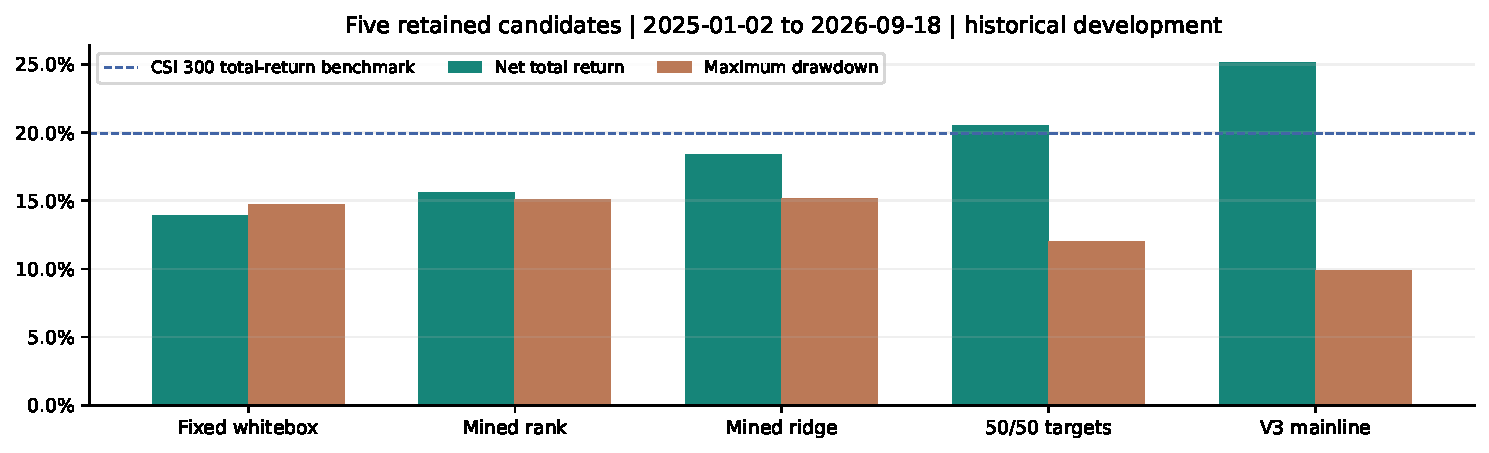
\includegraphics[width=.97\textwidth,height=52mm,keepaspectratio]{figures/v4_candidates.pdf}\end{center}
全收益基准19.94\%；三个白箱均未超过，固定50/50目标组合略超过但弱于主线。组合可能改善某些风险表现，却不能用较低回撤证明全面优越。全部候选、失败和修正前输出归档；这轮结论是\textbf{继续保留主线，辅助路线待前向观察}。

\page{8\quad 主线曲线、基准与执行压力}

\lead{相同起点和日期；价格、全收益与ETF代理明确区分。}
\begin{center}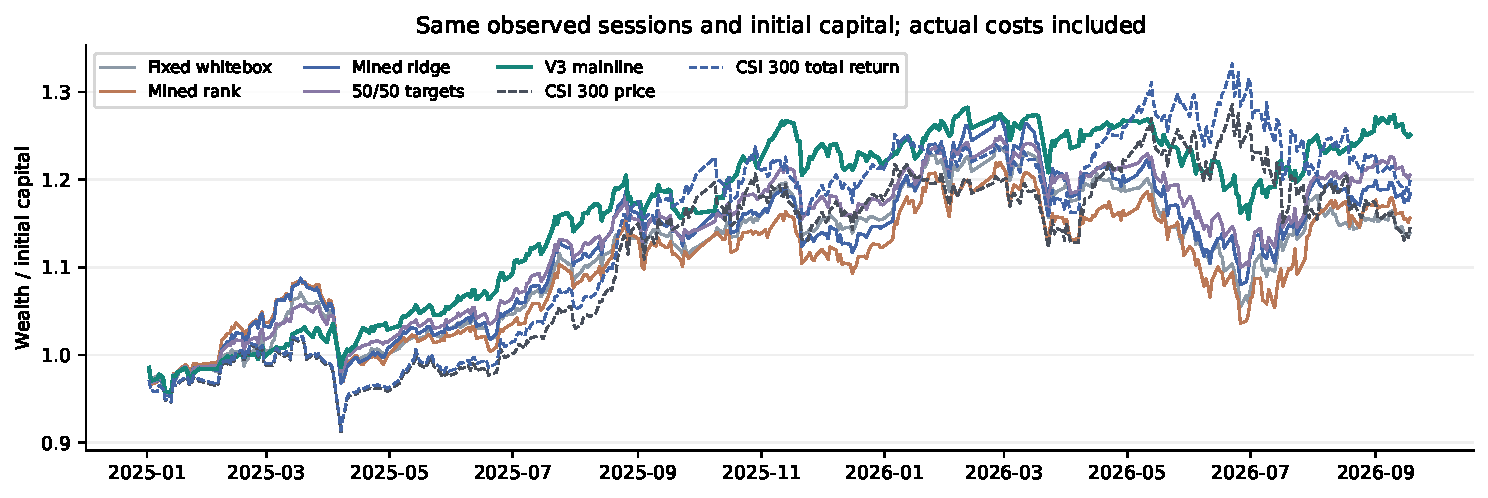
\includegraphics[width=.98\textwidth,height=66mm,keepaspectratio]{figures/v4_curves.pdf}\end{center}
策略从初始资金起算，指数用前一交易日收盘，保留首日损益；全收益指数计红利再投资，不能用ETF代理改名替代。主线收益25.13\%，分别超过价格14.55\%与全收益19.94\%；与全收益差5.19个百分点，相对财富增幅约4.33\%，两者不是同一口径。首次开盘起算价格基准结论不变，ETF复权代理另保留。
\subsection*{严格实际成交情景}
\begin{center}\small\begin{tabular}{lrrrr}\toprule
候选 & 严格净收益 & 夏普 & 严格回撤 & 实际成本(元)\\\midrule
V3主线LightGBM & 24.92\% & 1.260 & 9.71\% & 22,311.46\\
年度白箱Ridge & 18.15\% & 0.763 & 14.85\% & 23,058.61\\
主线/排名各50\% & 19.49\% & 0.971 & 11.35\% & 29,688.34\\
\bottomrule\end{tabular}\end{center}

独立最低佣金/税/滑点政策与基础买10bp、卖15bp不同，因此整手、现金与费用同时改变实际路径。严格情景并非单独增加整手约束的因果对照，亦不代表完整实盘可执行收益。
\subsection*{原压力和落后年份}
双倍基础费用主线22.48\%，信号延迟一日27.31\%；延迟更优未被据此改为默认。2023起连续运行44.09\%、最大回撤19.70\%，2024仍落后价格指数7.28个百分点。不能把累计领先描述为每年或每个市场状态都胜出。
\subsection*{基准排序修正}
厂商日线先按日期升序排列，再选首日前最近收盘。修正前指标归档，修正没有改变交易或预选；现用表与曲线采用一致边界。基准缺日拒绝，不插值，不从最早日期错误选取区间起点。

\page{9\quad 风险、资金归因与冻结观察}

\lead{分析已有路径，不虚构未发生的前向成绩。}
\begin{center}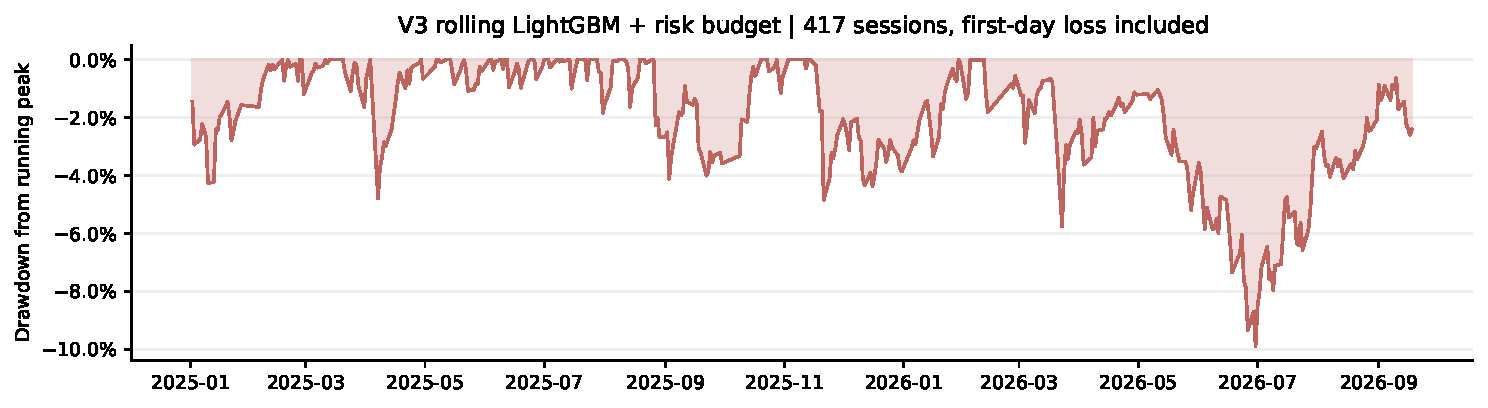
\includegraphics[width=.98\textwidth,height=40mm,keepaspectratio]{figures/v3_drawdown.pdf}\end{center}
同区间对比取严格交易日交集；内部缺日拒绝。切片第一日以此前净值起算，保留首日收益，高水位包含初始资金；它不是从现金重新开仓。月历包含首尾部分月份，60日滚动统计不补不足窗口；未恢复回撤不伪造恢复日期。静态现金情景$N^{mix}_t=wN_t+(1-w)$不再平衡、现金零利息，未重算规模与容量。
\subsection*{描述性资金账本归因}
\[
\Pi_i=SellCash_i-BuyCash_i-Cost_i+V_{i,T},\qquad \sum_i\Pi_i=NAV_T-NAV_0.
\]
已退出股票仍保留损益，各股贡献除以初始资金后相加等于组合收益。实际成本逐笔使用，未记录的佣金/税/滑点分项保持未知；按明确行业标签汇总时保留未知组。该功能是描述性现金流与期末估值归因，不冒充行业或因子的因果解释。
\subsection*{冻结身份与追加观察}
冻结策略ID、完整公式、年度参数、训练/执行配置、数据/代码哈希、UTC时点及最后已知交易日。只接受\texttt{observation\_date}>截止日；\texttt{signal\_asof}<成交日。独占新建文件，不覆盖旧计划；同内容重试幂等，冲突或前日插入拒绝，记录链经读回检查。
冻结前已经发生的新增历史属于历史补录；冻结后首先是纸面记录。\textbf{本地时钟、人工记录和哈希不能认证真实信息获取或账户成交}，不把旧净值贴成前向胜出。未来绩效仍待积累新数据。
\subsection*{指数增强的实测门槛}
组件需要当时真实可得的成分、权重及风险数据。当前缺完整历史指数权重，未运行真实增强策略；手工/合成权重只验证约束与流程，不发布其投资收益。指数方法准备、真实实测与交易授权分别报告。

\page{10\quad 外部接口、验收注入与复现}

\subsection*{LLM辅助的实际状态}
支持OpenAI兼容Chat Completions或本机Ollama；密钥临时传入，不写配置、结果或材料。发送明确研究问题和选定公式/证据；建议需DSL校验，再经评价器实测。\textbf{本次真实研究\texttt{llm\_called=false}，未发生真实模型请求}；离线说明标为确定性，模型文本标为未核验，不能制造IC或收益数字。
\subsection*{保留的原生接入与账户边界}
此前Qlib 0.9.7独立环境读取20股33,754条日线，8表达式对比269,554个数值；实际运行158项Alpha158配置，VWAP输入覆盖100\%。属于因子接口验证，未训练Qlib策略，未替换主成交账本。原接入证据保留，不由本次源码编写重新证明。

同花顺/SuperMind为文件桥：历史观察权重与代码导出、模拟成交CSV金额/重复核验、保存本地回执。账号/API未连接，未收到真实账户成交文件，未提交订单；历史权重不是今日信号，现金核对不等于盈利。
\subsection*{最终软件与界面验收}
最终测试：269项通过，1项跳过；以封存日志为准

界面核验：新页AppTest与独立浏览器交互通过；范围见evidence/ui\_v230
。测试数量和界面状态对应最终封存记录，记录范围之外的账户连接、真实指数增强与实盘成交没有据此验证。研究账本检查、数值前缀检查、UI交互和新增市场数据分别提供不同证据；公开聚合证据支持结果核对，真实训练与逐股查询仍依赖合法数据快照。
\subsection*{复现入口及可编辑材料}
\begin{itemize}
\item 双击\texttt{launch.cmd}，或按README安装固定依赖并启动Streamlit；缺私有快照时查看公开真实聚合证据。
\item 真实研究使用\texttt{scripts/run\_factor\_research.py}，新建输出身份；合法原始数据及训练缓存不随公开包发布。
\item 材料作者入口\texttt{scripts/build\_v230\_materials.py}只写源码和科学图；Beamer、报告、讲稿由独立XeLaTeX步骤编译。
\item \texttt{deck\_content.json}保持20条，正文18条20分钟、备份2条；同源生成可编辑PPTX与讲稿，图数据来自封存CSV。
\end{itemize}
\subsection*{来源与交付声明}
课程依据CF2026\_Project1.pdf；主线及历史诊断来自\texttt{evidence/research\_v2,v3}，新完整候选与压力来自\texttt{evidence/research\_v4}，原生Qlib及文件桥有独立状态证据。中证/Tushare用于数据与基准，CogAlpha只借鉴可检查表达式。源码、指标、数据身份和发布验收共同定位本版；材料准备、Git发布及Blackboard提交是各自状态，不以本报告生成替代。
\end{document}
